\documentclass[mathserif,spanish,10pt]{beamer}

\mode<presentation>{
  \usetheme{Madrid}
  \usecolortheme{whale}
  \setbeamertemplate{footline}[frame number]
  \setbeamertemplate{navigation symbols}{}
}

% ── Paquetes ────────────────────────────────────────────────────────────────
\usepackage{graphicx}
\usepackage{booktabs}
\usepackage{multirow}
\usepackage{caption}
\usepackage{subcaption}
\usefonttheme{professionalfonts}
\usepackage[justification=centering]{caption}
\usepackage{ragged2e}
\justifying
\usepackage[utf8]{inputenc}
\usepackage[spanish]{babel}
\usepackage{amsmath}
\usepackage{xcolor}
\usepackage{colortbl}
\usepackage{array}
\usepackage{tikz}
\usetikzlibrary{shapes,arrows,positioning}

% ── Colores IEEE-style ───────────────────────────────────────────────────────
\definecolor{navyblue}{RGB}{13,31,78}
\definecolor{accentteal}{RGB}{8,145,178}
\definecolor{lightblue}{RGB}{186,230,253}
\definecolor{kpigreen}{RGB}{22,163,74}
\definecolor{kpiorange}{RGB}{234,88,12}
\definecolor{rowsim}{RGB}{239,246,255}
\definecolor{rowexp}{RGB}{240,253,244}
\definecolor{rowhdr}{RGB}{13,31,78}

% ── Macros ───────────────────────────────────────────────────────────────────
\newcommand{\highlight}[1]{\textbf{\color{accentteal}#1}}
\newcommand{\good}[1]{\textbf{\color{kpigreen}#1}}
\newcommand{\warn}[1]{\textbf{\color{kpiorange}#1}}

% Estilo caption IEEE dentro de beamer
\captionsetup{
  font=scriptsize,
  labelfont=bf,
  labelsep=period,
  justification=centering
}

% ── Metadatos ────────────────────────────────────────────────────────────────
\title[Lab~3 · Grúa]{Identificación y Control de un Sistema de Grúa}
\subtitle{Grupo~B — Laboratorio de Control Automático}
\author[Castro, Chavarría, Segura]{%
  E.\,Castro \and D.\,Chavarría \and E.\,Segura}
\institute[TEC]{%
  Instituto Tecnológico de Costa Rica\\
  Escuela de Ingeniería Electrónica}
\date{\today}

% ════════════════════════════════════════════════════════════════════════════
\begin{document}

% ── Portada ──────────────────────────────────────────────────────────────────
\begin{frame}[plain]
  \titlepage
\end{frame}

% ── Tabla de contenidos ──────────────────────────────────────────────────────
\begin{frame}{Contenido}
  \tableofcontents[
    sectionstyle=show,
    subsectionstyle=show/shaded/hide,
    subsubsectionstyle=hide
  ]
\end{frame}

% ── Agenda automática al inicio de cada sección ──────────────────────────────
\AtBeginSection[]{
  \begin{frame}{Contenido}
    \tableofcontents[
      currentsection,
      sectionstyle=show/shaded,
      subsectionstyle=show/shaded/hide
    ]
  \end{frame}
}

%=============================================================================
\section{Objetivo}
%=============================================================================

\begin{frame}{Objetivo}
\begin{columns}[T]
  \column{0.55\textwidth}
  \begin{block}{Metas del laboratorio}
    \begin{itemize}
      \item Identificar experimentalmente la planta carro-péndulo.
      \item Obtener modelo \textbf{SIMO} promedio en espacio de estados.
      \item Diseñar y evaluar controladores \textbf{REI}:
        \begin{itemize}
          \item \textit{Pole Placement} (PP)
          \item LQR con regla de Bryson
        \end{itemize}
      \item Comparar simulación vs.\ experimento.
      \item Evaluar atenuación de oscilación del péndulo.
    \end{itemize}
  \end{block}

  \column{0.42\textwidth}
  \begin{block}{Métricas de evaluación}
    \vspace{0.2cm}
    \centering
    \small
    \rowcolors{2}{rowsim}{white}
    \begin{tabular}{cl}
      \hline
      \rowcolor{rowhdr}
      \color{white}\textbf{Símbolo} & \color{white}\textbf{Descripción} \\
      \hline
      $t_s$    & Settling Time \\[4pt]
      $M_p$    & OverShoot (\%) \\[4pt]
      $e_{ss}$ & Error estacionario \\[4pt]
      $\theta$ & Oscilación del péndulo \\
      \hline
    \end{tabular}
  \end{block}
\end{columns}
\end{frame}

%=============================================================================
\section{Identificación del sistema}
%=============================================================================

\subsection{Setup experimental}

\begin{frame}{Setup Experimental}
\begin{columns}[T]
  \column{0.52\textwidth}
  \begin{block}{Plataforma}
    \begin{itemize}
      \item Carro accionado por motor DC con transmisión polea-banda.
      \item Péndulo acoplado al carro.
      \item Encoders ópticos incrementales: posición~$p$ y ángulo~$\theta$.
      \item Señal de excitación: trapezoidal $\approx 7.5\,\text{V}$.
      \item Periodo de muestreo: $T_s = 20\,\text{ms}$.
    \end{itemize}
  \end{block}

  \begin{block}{Criterio de selección de muestras}
    \small
    Se escogieron 4 conjuntos de datos.\\
    Criterio: mínimo coeficiente de variación (CV) sobre los parámetros identificados.
  \end{block}

\end{columns}
\end{frame}

%─────────────────────────────────────────────────────────────────────────────
\subsection{Parámetros identificados}

\begin{frame}{Parámetros Identificados — Posición y Ángulo}
\begin{columns}[T]

  % ── COLUMNA IZQUIERDA: POSICIÓN DEL CARRO ─────────────────────────────────
  \column{0.48\textwidth}
  {\centering\small\color{navyblue}\textbf{Posición del carro} $G_p(s)$\par}
  \vspace{4pt}
  
  \begin{table}
    \centering
    \scriptsize
    \rowcolors{2}{rowsim}{white}
    \begin{tabular}{lcc}
      \hline
      \rowcolor{rowhdr}
      \color{white}\textbf{Muestra} &
      \color{white}$K$ &
      \color{white}$a_x$ \\
      \hline
      grua1 & 0.2493 & 10.41 \\
      grua2 & 0.2542 & 10.50 \\
      grua5 & 0.2546 & 10.44 \\
      grua6 & 0.2611 & 10.69 \\
      \rowcolor{accentteal!20}
      \textbf{Promedio} & \textbf{0.2548} & \textbf{10.51} \\
      \hline
    \end{tabular}
  \end{table}

  \vspace{-2pt}
  \begin{block}{Modelo promedio $G_p(s)$}
    \centering\scriptsize
    \[
      G_p(s) = \frac{0.2548}{s^2 + 10.51s + 8.66\times10^{-7}}
    \]
  \end{block}

  \vspace{-2pt}
  {\centering\fontsize{7pt}{8pt}\selectfont
  CV$(K)=1.67\%$ \quad CV$(a_x)=0.99\%$\\
  $\Rightarrow$ Modelo estable y confiable.\par}

  % ── COLUMNA DERECHA: ÁNGULO DEL PÉNDULO ───────────────────────────────────
  \column{0.48\textwidth}
  {\centering\small\color{navyblue}\textbf{Ángulo del péndulo} $G_\theta(s)$\par}
  \vspace{4pt}

  \begin{table}
    \centering
    \scriptsize
    \rowcolors{2}{rowsim}{white}
    \begin{tabular}{lccc}
      \hline
      \rowcolor{rowhdr}
      \color{white}\textbf{Mues.} &
      \color{white}$\omega_n$ &
      \color{white}$\zeta$ &
      \color{white}$K$ \\
      \hline
      grua1 & 5.9447 & 0.0016 & $-$0.0141 \\
      grua2 & 5.9439 & 0.0013 & $-$0.0112 \\
      grua5 & 5.9464 & 0.0014 & $-$0.0135 \\
      grua6 & 5.9464 & 0.0013 & $-$0.0145 \\
      \rowcolor{accentteal!20}
      \textbf{Prom.} & \textbf{5.9454} & \textbf{0.0014} & \textbf{$-$0.0133} \\
      \hline
    \end{tabular}
  \end{table}

  \vspace{-2pt}
  \begin{block}{Modelo promedio $G_\theta(s)$}
    \centering\scriptsize
    \[
      G_\theta(s) = \frac{-0.3858s - 0.4703}{s^2 + 0.01685s + 35.35}
    \]
  \end{block}

  \vspace{-2pt}
  {\centering\fontsize{7pt}{8pt}\selectfont
  CV$(\omega_n)<0.05\% \Rightarrow$ Muy consistente.\\
  Subamortiguado: $\zeta\approx0.0014$.\par}

\end{columns}
\end{frame}
%─────────────────────────────────────────────────────────────────────────────
\subsection{Modelo SIMO en espacio de estados}

\begin{frame}{Modelo SIMO en Espacio de Estados}
\begin{columns}[T]
  \column{0.54\textwidth}
  \vspace{-4pt}
  \[
    \mathbf{x}^T = \begin{bmatrix} p & \theta & \dot{p} & \dot{\theta} \end{bmatrix}
  \]
  \[
    A = \begin{bmatrix}
          0 & 0 & 1 & 0 \\
          0 & 0 & 0 & 1 \\
          0 & 0 & -10.51 & 0 \\
          0 & -35.35 & 0 & -0.0169
        \end{bmatrix}
  \]
  \[
    B = \begin{bmatrix} 0 \\ 0 \\ 0.2548 \\ -0.3858 \end{bmatrix}, \quad
    C = \begin{bmatrix} 1 & 0 & 0 & 0 \end{bmatrix}
  \]

  \column{0.43\textwidth}
  \begin{block}{Observaciones clave}
    \scriptsize
    \begin{itemize}
      \item Sistema de \textbf{4.º orden}: doble integrador en posición.
      \item Acoplamiento dinámico: $A_{42}=-35.35$ (péndulo $\leftrightarrow$ carro).
      \item Salida única $p$ dando una estructura \textbf{SIMO}.
      \item Péndulo casi sin amortiguamiento: $a_{44}=-0.0169\approx 0$.
    \end{itemize}
  \end{block}

  \begin{block}{Controlabilidad}
    \centering\small
    $\operatorname{rank}(\mathcal{M}_c) = 4$\\[2pt]
    Sistema totalmente controlable.
  \end{block}
\end{columns}
\end{frame}

%=============================================================================
\section{Diseño de controladores REI}
%=============================================================================

\begin{frame}{Estrategia REI — Marco Común}
\begin{columns}[T]
  \column{0.50\textwidth}
  \begin{block}{Integral State Feedback (ISF)}
    \begin{itemize}
      \item Estado integral del error: $\dot{x}_I = r - C_r\,\mathbf{x}$
      \item Ley de control: $u = -K\mathbf{x} + K_I\,x_I$
      \item Sistema \textbf{aumentado} de 5 estados.
      \item $\operatorname{rank}(\hat{\mathcal{M}}_c) = 5$ \good{$\checkmark$}
    \end{itemize}
  \end{block}

  \begin{block}{Beneficios del esquema ISF}
    \scriptsize
    \begin{itemize}
      \item $e_{ss}=0$ garantizado ante entrada escalón.
      \item Polos de lazo cerrado asignables libremente.
      \item Atenuación activa de la oscilación del péndulo.
    \end{itemize}
  \end{block}

  \column{0.46\textwidth}
  \begin{block}{Técnicas evaluadas}
    \centering\small
    \begin{tabular}{ll}
      \toprule
      Técnica & Criterio de diseño \\
      \midrule
      Pole Placement & Ubicación manual \\
      LQR & Optimización $J$ \\
      \bottomrule
    \end{tabular}
  \end{block}
\end{columns}
\end{frame}

%─────────────────────────────────────────────────────────────────────────────
\subsection{Pole Placement}

\begin{frame}{Pole Placement — Diseño}
\begin{columns}[T]
  \column{0.50\textwidth}
  \begin{block}{Metodología}
    \begin{enumerate}
      \item Construir sistema \textbf{aumentado} (4+1 estados).
      \item Seleccionar \textbf{5 polos deseados} en $\mathbb{C}^-$.
      \item Calcular $\hat{K}=\begin{bmatrix}K & K_I\end{bmatrix}$ con \texttt{place()} en MATLAB.
      \item Verificar dinámica de lazo cerrado.
    \end{enumerate}
  \end{block}

  \begin{alertblock}{Criterios de selección de polos}
    \scriptsize
    \begin{itemize}
      \item Par dominante: $t_s$ y $M_p$ deseados.
      \item Polos rápidos: $\times 3$ más rápidos que dominantes.
      \item Polo integral suficientemente rápido.
      \item Evitar cancelación con ceros del modelo.
    \end{itemize}
  \end{alertblock}

  \column{0.46\textwidth}
  \begin{exampleblock}{Polos de lazo cerrado seleccionados}
    \scriptsize
    \centering
    \begin{tabular}{cc}
      \toprule
      Polo & Valor \\
      \midrule
      $p_{1,2}$ & $-\square \pm j\square$ \\
      $p_3$     & $-\square$ \\
      $p_4$     & $-\square$ \\
      $p_5$     & $-\square$ \\
      \bottomrule
    \end{tabular}\\[4pt]
    \textit{\tiny Completar con valores de diseño.}
  \end{exampleblock}
\end{columns}
\end{frame}

%─────────────────────────────────────────────────────────────────────────────

\begin{frame}{Pole Placement — Simulación vs.\ Experimento}
\begin{columns}[T]

  \column{0.48\textwidth}
  {\centering\small\color{navyblue}\textbf{Simulación}\par}
  \vspace{4pt}
  \begin{figure}
    \centering
    \fbox{\rule{0pt}{2.2cm}\rule{4.2cm}{0pt}}
    \caption{Posición $p(t)$ — Simulación PP.}
    \label{fig:pp_sim}
  \end{figure}
  \vspace{-4pt}
  \begin{table}
    \centering
    \caption{KPIs — Simulación PP.}
    \label{tab:kpi_pp_sim}
    \scriptsize
    \rowcolors{1}{rowsim}{}
    \begin{tabular}{lc}
      \toprule
      Métrica & Valor \\
      \midrule
      $t_s$ (s)      & $\square$ \\
      $M_p$ (\%)     & $\square$ \\
      $e_{ss}$        & $\square$ \\
      Osc.\ péndulo  & $\square$ \\
      \bottomrule
    \end{tabular}
  \end{table}

  \column{0.48\textwidth}
  {\centering\small\color{navyblue}\textbf{Experimento}\par}
  \vspace{4pt}
  \begin{figure}
    \centering
    \fbox{\rule{0pt}{2.2cm}\rule{4.2cm}{0pt}}
    \caption{Posición $p(t)$ — Experimental PP.}
    \label{fig:pp_exp}
  \end{figure}
  \vspace{-4pt}
  \begin{table}
    \centering
    \caption{KPIs — Experimental PP.}
    \label{tab:kpi_pp_exp}
    \scriptsize
    \rowcolors{1}{rowexp}{}
    \begin{tabular}{lc}
      \toprule
      Métrica & Valor \\
      \midrule
      $t_s$ (s)      & $\square$ \\
      $M_p$ (\%)     & $\square$ \\
      $e_{ss}$        & $\square$ \\
      Osc.\ péndulo  & $\square$ \\
      \bottomrule
    \end{tabular}
  \end{table}

\end{columns}
\vspace{2pt}
{\centering\tiny\color{gray}\textit{Referencia: escalón de 0.5\,m. Completar con datos experimentales.}\par}
\end{frame}

%─────────────────────────────────────────────────────────────────────────────
\subsection{LQR}

\begin{frame}{LQR — Regla de Bryson}
\begin{columns}[T]
  \column{0.50\textwidth}
  \begin{block}{Criterio de diseño}
    \[
      J = \int_0^\infty \!\bigl(\mathbf{x}^TQ\mathbf{x} + u^TRu\bigr)\,dt
    \]
    \[
      Q_{ii} = \frac{1}{x_{i,\max}^2}, \qquad
      R = \frac{1}{u_{\max}^2}
    \]
  \end{block}

  \vspace{4pt}
  \begin{block}{Ganancias obtenidas}
    \centering\scriptsize
    \[
      K = \begin{bmatrix}80.04 & {-}23.19 & 7.13 & {-}7.01\end{bmatrix}
    \]
    \[
      K_I = -40.0
    \]
    \textbf{Polos LC:}\;
    $-10.47,\;{-}1.50\pm 6.12j,\;{-}0.79\pm 0.49j$
  \end{block}

  \column{0.46\textwidth}
  \begin{table}
    \centering
    \caption{Pesos de Bryson para el LQR.}
    \label{tab:bryson}
    \scriptsize
    \rowcolors{2}{rowsim}{white}
    \begin{tabular}{p{1.5cm}cc}
      \rowcolor{rowhdr}
      \color{white}\textbf{Estado} &
      \color{white}$x_{\max}$ &
      \color{white}$Q_{ii}$ \\
      \midrule
      Posición $p$         & 0.112\,m     & 80.0 \\
      Ángulo $\theta$      & 0.209\,rad   & 23.0 \\
      $\dot{p}$            & 1.0\,m/s     & 1.0 \\
      $\dot{\theta}$       & 0.354\,rad/s & 8.0 \\
      Error int.\ $\xi$    & 0.158\,m·s   & 40.0 \\
      Control $u$          & 1.0\,V       & $R=1.0$ \\
    \end{tabular}
  \end{table}
\end{columns}
\end{frame}

%─────────────────────────────────────────────────────────────────────────────

\begin{frame}{LQR — Posicón del carro: Simulación vs.\ Experimento}
\begin{columns}[T]

  \column{0.48\textwidth}
  {\centering\small\color{navyblue}\textbf{Simulación}\par}
  \vspace{4pt}
  \begin{figure}
    \centering
    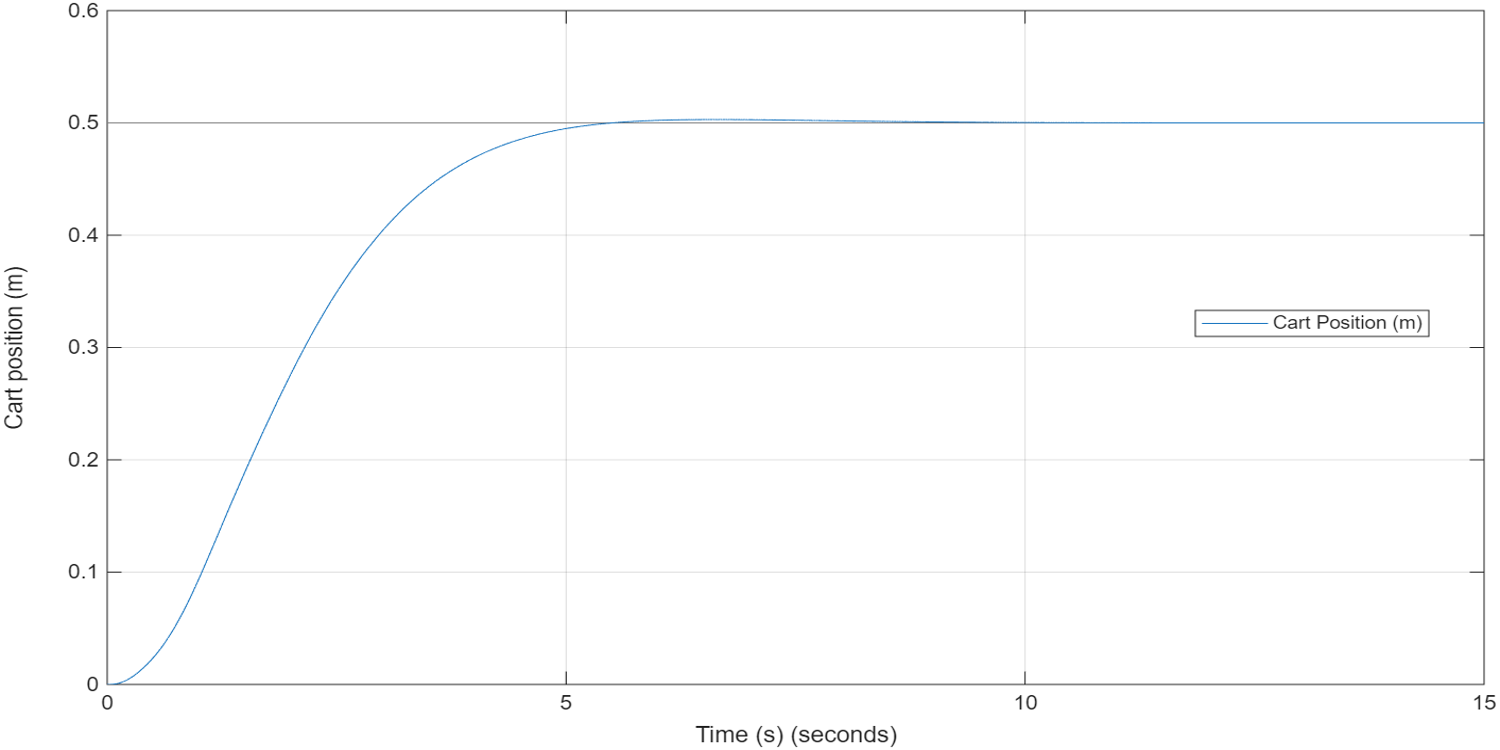
\includegraphics[width=0.95\linewidth]{Figures/grafica_carrito_s.png}
    \caption{Respuesta de simulación de posición usando LQR.}
    \label{fig:lqr_angle_sim}
  \end{figure}
  \vspace{-4pt}
  \begin{table}
    \centering
    \caption{Métricas deposición de la simulación con LQR.}
    \label{tab:kpi_lqr_ang_sim}
    \scriptsize
    \begin{tabular}{lc}
      \toprule Métrica & Valor \\ \midrule
      $t_s$ (s)  & 4.701 \\
      $M_p$ (\%) & 0.601 \\
      $e_{ss}$   & 0 \\
      \bottomrule
    \end{tabular}
  \end{table}

  \column{0.48\textwidth}
  {\centering\small\color{navyblue}\textbf{Experimento}\par}
  \vspace{4pt}
  \begin{figure}
    \centering
    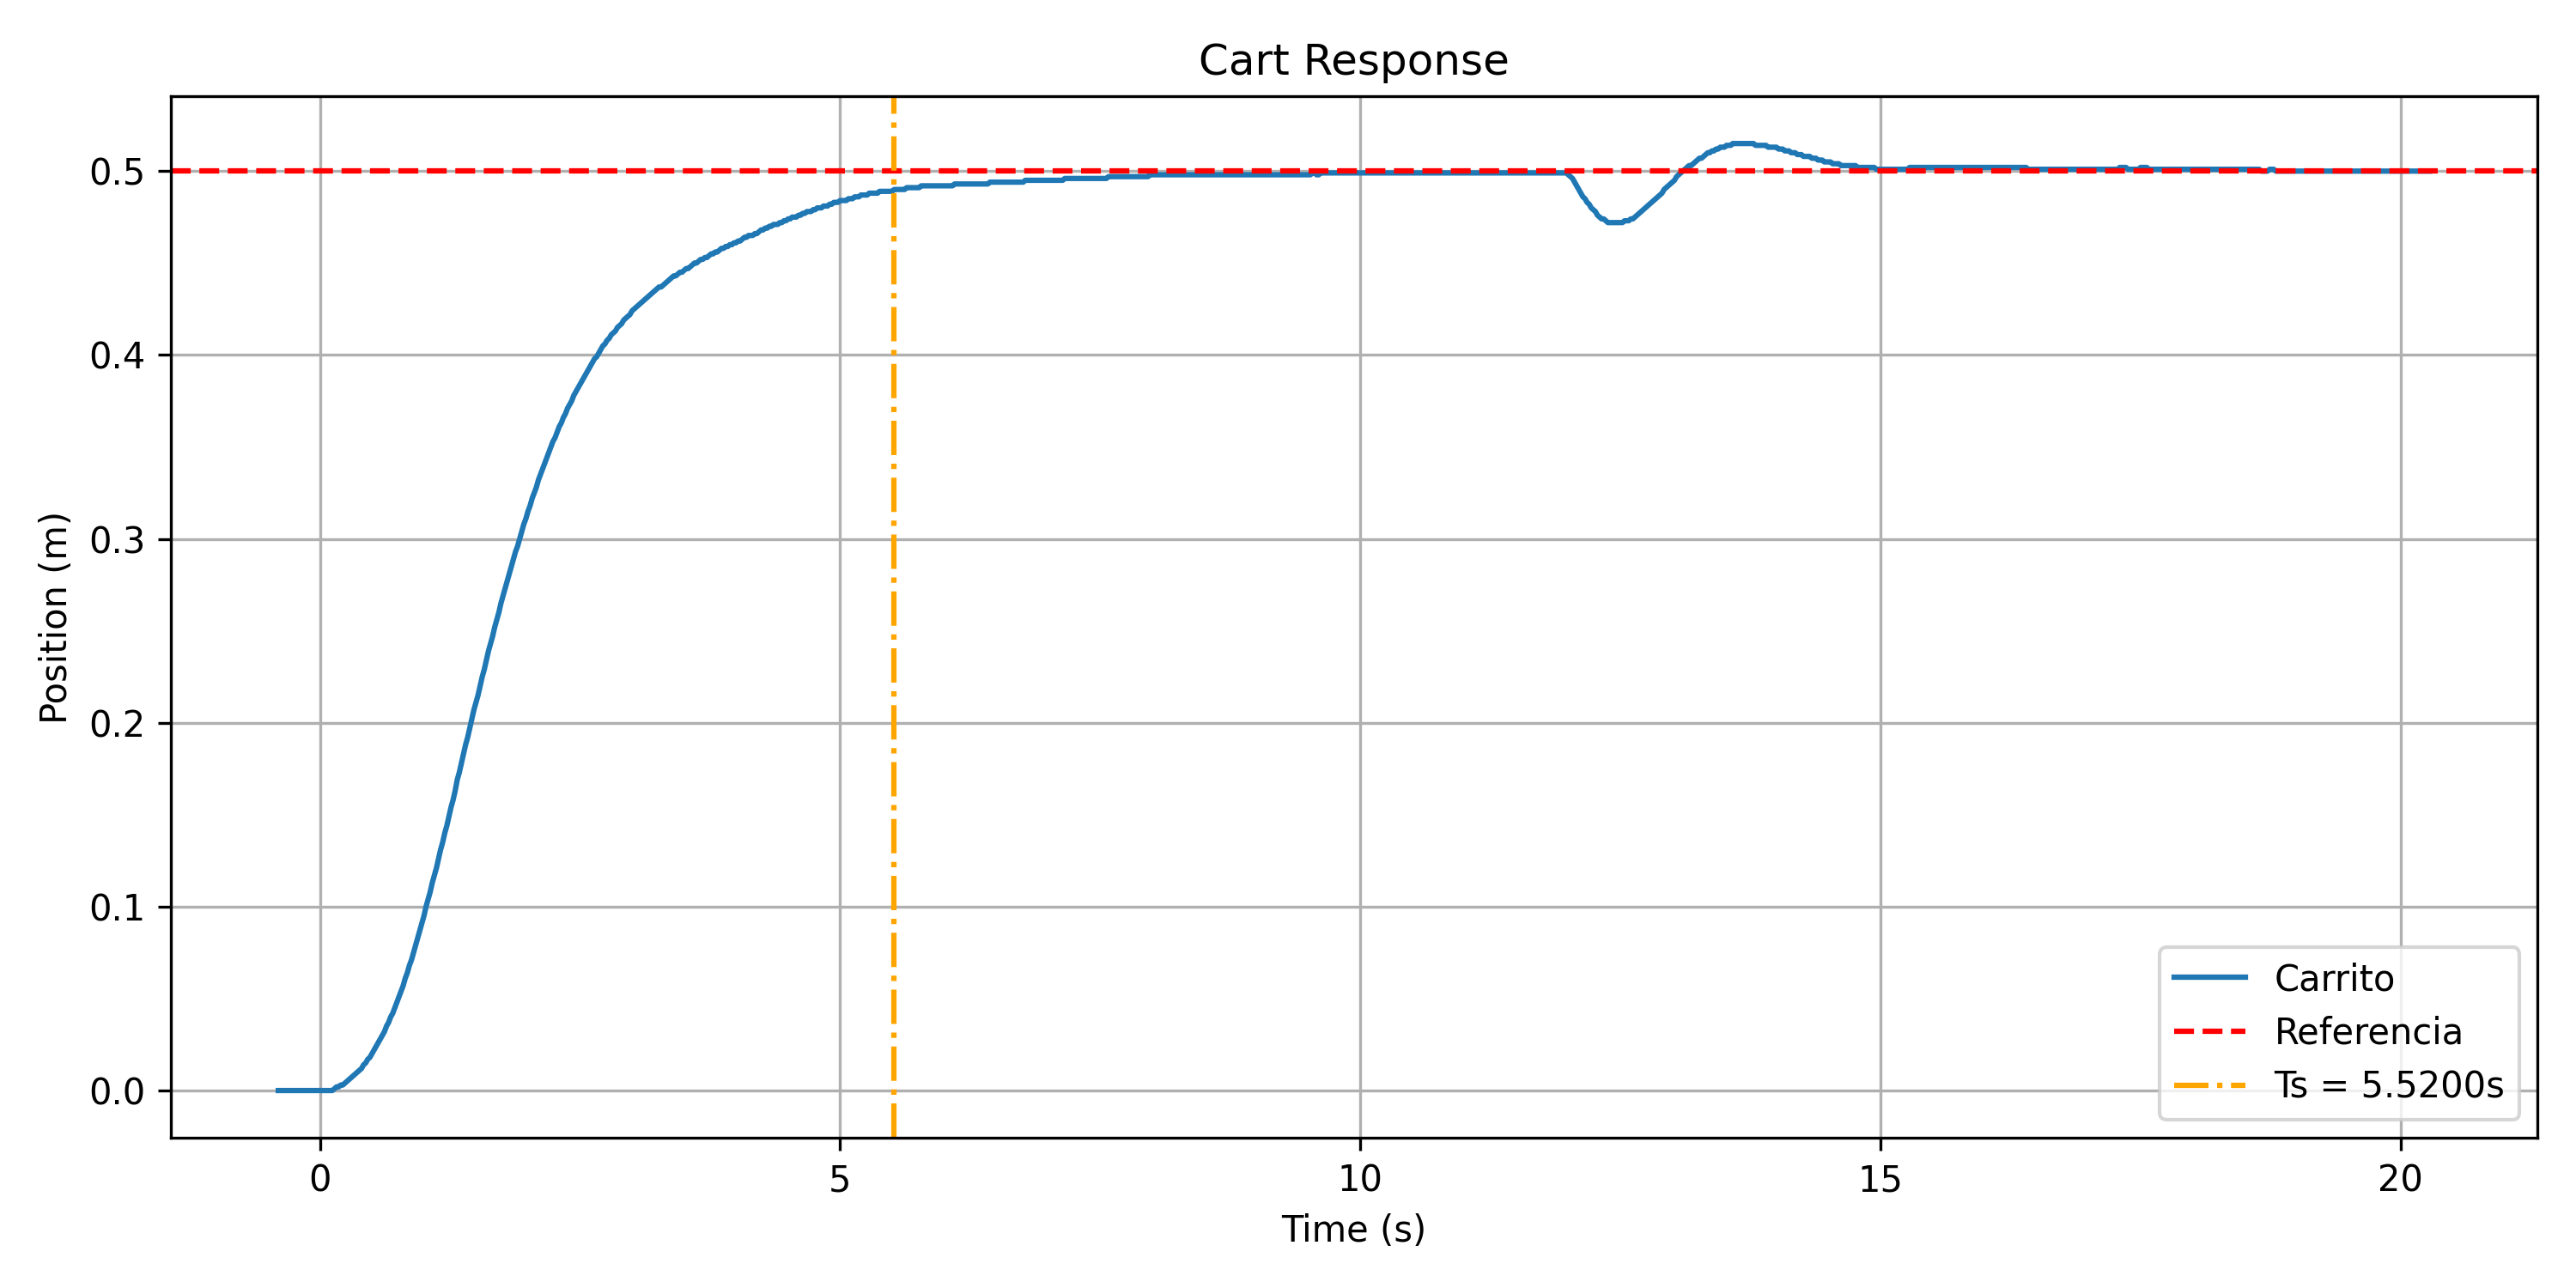
\includegraphics[width=0.95\linewidth]{Figures/grafica_carrito.png}
    \caption{Respuesta experimental de posición usando LQR.}
    \label{fig:lqr_angle_exp}
  \end{figure}
  \vspace{-4pt}
  \begin{table}
    \centering
    \caption{Métricas deposición del experimento con LQR.}
    \label{tab:kpi_lqr_ang_exp}
    \scriptsize
    \begin{tabular}{lc}
      \toprule Métrica & Valor \\ \midrule
      $t_s$ (s)  & 5.25 \\
      $M_p$ (\%) & 0 \\
      $e_{ss}$   & 0 \\
      \bottomrule
    \end{tabular}
  \end{table}

\end{columns}
\end{frame}

%─────────────────────────────────────────────────────────────────────────────

\begin{frame}{LQR — Ángulo del péndulo: Simulación vs.\ Experimento}
\begin{columns}[T]

  \column{0.48\textwidth}
  {\centering\small\color{navyblue}\textbf{Simulación}\par}
  \vspace{4pt}
  \begin{figure}
    \centering
    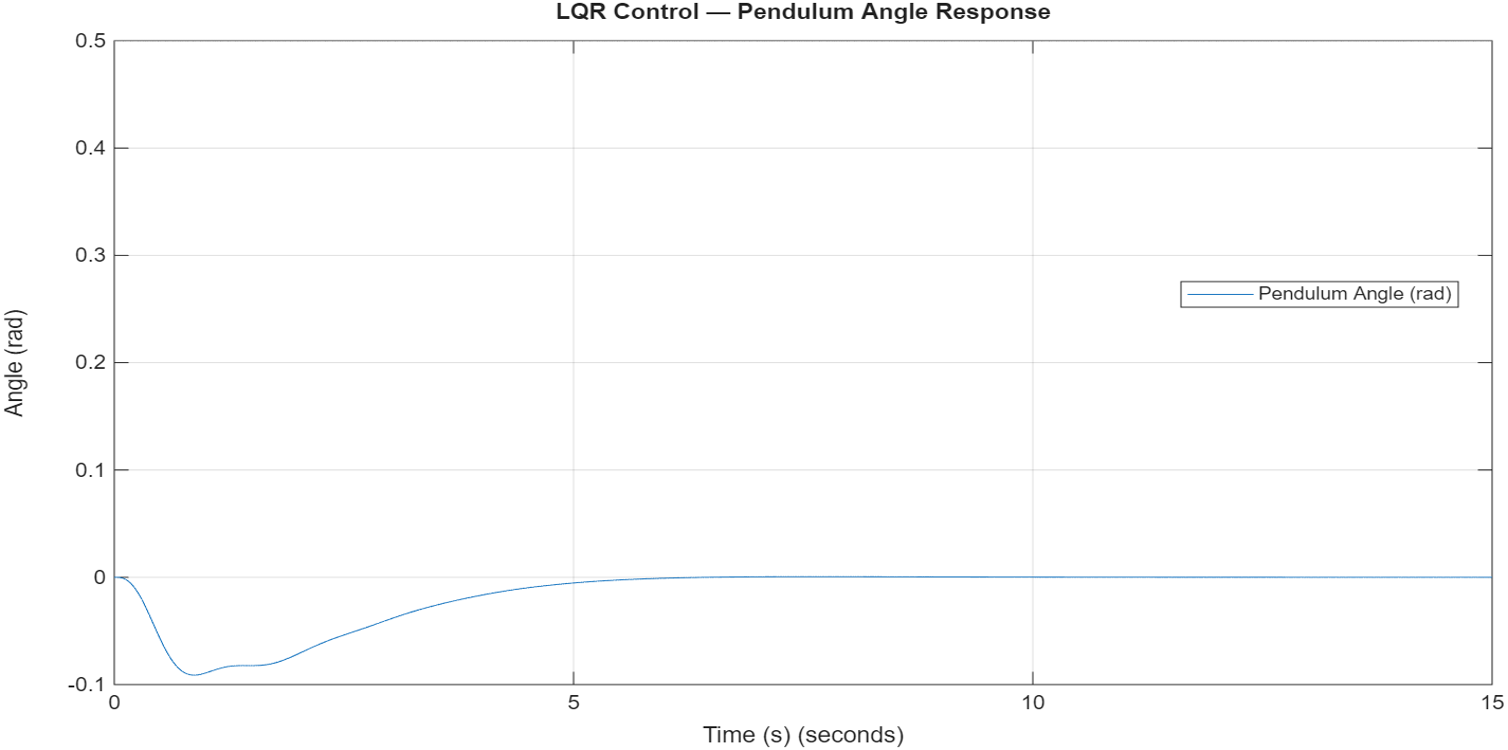
\includegraphics[width=0.95\linewidth]{Figures/grafica_angle_s.png}
    \caption{Respuesta de simulación de ángulo usando LQR.}
    \label{fig:lqr_pos_sim}
  \end{figure}
  \vspace{-4pt}
  \begin{table}
    \centering
    \caption{Métricas de ángulo de la simulación con LQR.}
    \label{tab:kpi_lqr_pos_sim}
    \scriptsize
    \begin{tabular}{lc}
      \toprule Métrica & Valor \\ \midrule
      $\theta(t)$ (s)  & 0 rads \\
      \bottomrule
    \end{tabular}
  \end{table}

  \column{0.48\textwidth}
  {\centering\small\color{navyblue}\textbf{Experimento}\par}
  \vspace{4pt}
  \begin{figure}
    \centering
    
\includegraphics[width=0.95\linewidth]{Figures/grafica_angulo.png}
    \caption{Respuesta experimental de ángulo usando LQR.}
    \label{fig:lqr_pos_exp}
  \end{figure}
  \vspace{-4pt}
  \begin{table}
    \centering
    \caption{Métricas de ángulo del experimento con LQR.}
    \label{tab:kpi_lqr_pos_exp}
    \scriptsize
    \begin{tabular}{lc}
      \toprule Métrica & Valor \\ \midrule
      $\theta(t)$ (s)  & 0.17 rads \\
      \bottomrule
    \end{tabular}
  \end{table}

\end{columns}
\end{frame}

%=============================================================================
\section{Comparativa}
%=============================================================================

\begin{frame}{Comparativa Final — PP vs.\ LQR}

  \begin{table}
    \centering
    \caption{Resumen de métricas de desempeño para ambos controladores.}
    \label{tab:comparativa}
    \small
    \begin{tabular}{llcccc}
      \hline
      \rowcolor{rowhdr}
      \color{white}\textbf{Controlador} &
      \color{white}\textbf{Cond.} &
      \color{white}$t_s$ (s) &
      \color{white}$M_p$ (\%) &
      \color{white}$e_{ss}$ &
      \color{white}Osc.\ pénd. \\
      \hline

      & Sim. & $-$ & $-$ & $-$ & $-$ \\
      \sidebyside{\multirow{-2}{*}{Pole Placement}}
      & Exp. & $-$ & $-$ & $-$ & $-$ \\
      \hline
      \rowcolor{rowsim}
      & Sim. & 4.701 & 0.601 & 0 & Atenuada \\
      \rowcolor{rowsim}
      \sidebyside{\multirow{-2}{*}{LQR}}
      & Exp. & 5.25  & 0     & 0 & Atenuada \\
      \hline
    \end{tabular}
\end{table}

  \vspace{4pt}
  \begin{columns}[T]
    \column{0.48\textwidth}
    \begin{block}{Análisis cuantitativo (LQR)}
      \scriptsize
      \begin{itemize}
        \item $\Delta t_s = +0.55\,\text{s}$ (+11.7\%) entre sim.\ y exp.
        \item $\Delta M_p = -0.60\%$: el sistema físico es más amortiguado.
        \item $e_{ss} = 0$ garantizado por acción integral.
        \item Oscilación del péndulo atenuada en ambas condiciones.
      \end{itemize}
    \end{block}

    \column{0.48\textwidth}
    \begin{block}{Ventajas y limitaciones}
      \scriptsize
      \centering
      \vspace{4pt}
      \begin{tabular}{p{0.9cm}p{1.5cm}p{1.5cm}}
        \toprule
        & \textbf{PP} & \textbf{LQR} \\
        \midrule
        Diseño       & Intuitivo    & Sistemático \\
        Esfuerzo	 & No regulado  & Minimizado \\
        Ajuste       & Manual       & Bryson \\
        \bottomrule
      \end{tabular}
    \end{block}
  \end{columns}
\end{frame}

%=============================================================================
\section{Conclusiones}
%=============================================================================

\begin{frame}{Conclusiones}
  \begin{enumerate}
    \item Se identificó la planta grúa obteniendo un modelo SIMO de 4.º orden con
          \good{CV\,$<\,$2\,\%} en todos los parámetros, lo que garantiza confiabilidad del modelo.

    \item El controlador \textbf{LQR} cumplió las especificaciones de diseño:
          \[
            t_s^{\text{sim}}=4.70\,\text{s},\quad
            M_p^{\text{sim}}=0.60\,\%,\quad
            t_s^{\text{exp}}=5.25\,\text{s},\quad
            M_p^{\text{exp}}=0\,\%,\quad
            e_{ss}=0.
          \]

    \item La \textbf{acción integral} del esquema ISF garantizó error estacionario nulo.

    \item Las diferencias entre simulación y experimento se atribuyen a:\\
          \textit{fricción no modelada · zona muerta · saturación del actuador}.

    \item La ausencia de sobreimpulso experimental indica mayor amortiguamiento
          físico que el del modelo linealizado.
  \end{enumerate}
\end{frame}

%─────────────────────────────────────────────────────────────────────────────
\subsection{Recomendaciones}

\begin{frame}{Recomendaciones}
\begin{columns}[T]
  \column{0.50\textwidth}
  \begin{block}{Identificación}
    \begin{itemize}
      \item Incorporar más conjuntos experimentales para reducir CV.
      \item Aplicar criterios estadísticos formales (IQR, Chauvenet) para descartar atípicos.
    \end{itemize}
  \end{block}

  \begin{block}{Modelado}
    \begin{itemize}
      \item Incluir efectos no lineales:\\
            fricción · zona muerta · saturación.
    \end{itemize}
  \end{block}

  \column{0.46\textwidth}
  \begin{block}{Control}
    \begin{itemize}
      \item Ajustar pesos de Bryson conservadoramente para reducir esfuerzo de control.
      \item Explorar técnicas robustas ($H_\infty$, LQG) para mejor atenuación del péndulo.
      \item Agregar realimentación de $\theta$ como salida secundaria para control explícito del ángulo.
    \end{itemize}
  \end{block}
\end{columns}
\end{frame}

%=============================================================================
\section{Bibliografía}
%=============================================================================

\begin{frame}[allowframebreaks]{Bibliografía}
  \footnotesize
  \begin{thebibliography}{9}
    \bibitem{ogata}
      K.\,Ogata,
      \emph{Modern Control Engineering}, 5th~ed.
      Prentice Hall, 2010.
    \bibitem{ljung}
      L.\,Ljung,
      \emph{System Identification: Theory for the User}, 2nd~ed.
      Prentice Hall, 1999.
    \bibitem{anderson}
      B.\,D.\,O.\,Anderson y J.\,B.\,Moore,
      \emph{Optimal Control: Linear Quadratic Methods}.
      Prentice Hall, 1990.
    \bibitem{franklin}
      G.\,F.\,Franklin, J.\,D.\,Powell y M.\,L.\,Emami-Naeini,
      \emph{Feedback Control of Dynamic Systems}, 4th~ed.
      Prentice Hall, 1998.
    \bibitem{mathworks}
      MathWorks,
      \emph{System Identification Toolbox — Documentation}.
      Disponible en: \texttt{https://www.mathworks.com/help/ident/}
  \end{thebibliography}
\end{frame}

\end{document}